\documentclass[english,serif,mathserif,xcolor=pdftex,dvipsnames,table]{beamer}
\usepackage{gc3}

\title{%
  The \texttt{ParallelTaskCollection}
}
\author[Antonio Messina]{%
  GC3: Grid Computing Competence Center, \\
  University of Zurich
}
\date{Oct.~2, 2012}

\begin{document}

% title frame
\maketitle


\begin{frame}[fragile]
  \frametitle{Running jobs in parallel}

  \texttt{ParallelTaskCollection} provides an interface for
  running jobs in parallel.
  
  \+
  \begin{center}
    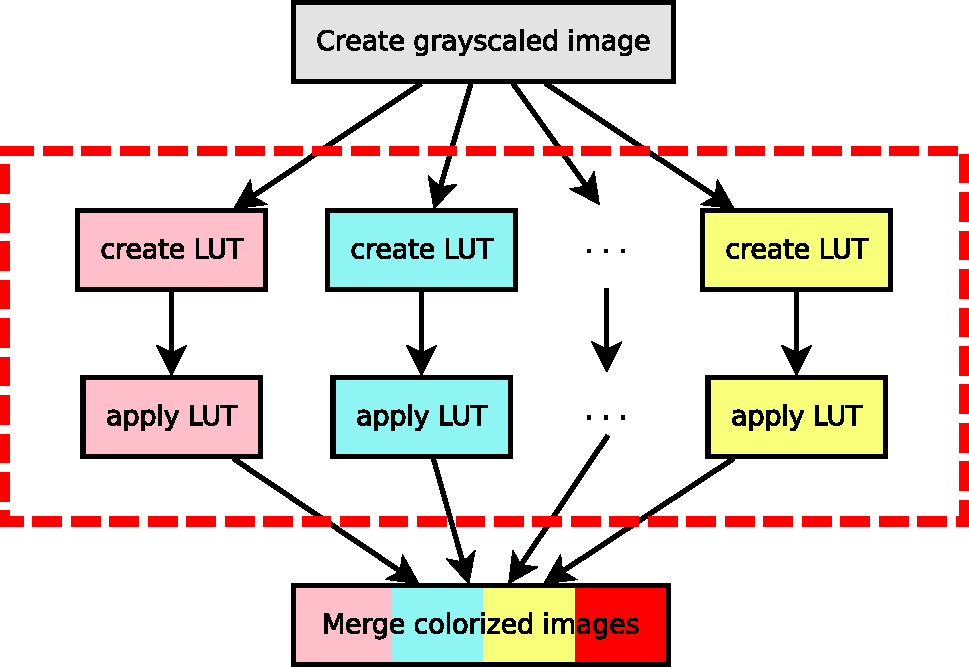
\includegraphics[width=0.75\textwidth]{fig/warholize-wkf2}
  \end{center}
\end{frame}


\begin{frame}[fragile]
  \frametitle{\texttt{ParallelTaskCollection} - example}
  \begin{lstlisting}[basicstyle=\tt\scriptsize]
from gc3libs.workflow import @\HL{ParallelTaskCollection}@

class ParallelHello(@\HL{ParallelTaskCollection}@):
    def __init__(self, hwstring, ncopies, **extra):
        tasks = []
        for i in range(ncopies):
            extra_args = extra.copy()
            extra_args['output_dir'] += ".%d" % i
            task.append(
                GHelloWorld(
                    hwstring,
                    **extra_args))
        # This is IMPORTANT!!!
        ParallelTaskCollection.__init__(self, tasks, **extra)
  \end{lstlisting}
\end{frame}



\begin{frame}[fragile]
  \frametitle{\texttt{ParallelTaskCollection} - example}
  \begin{lstlisting}[basicstyle=\tt\scriptsize]
from gc3libs.workflow import ParallelTaskCollection

class ParallelHello(ParallelTaskCollection):
    def __init__(self, hwstring, ncopies, @\HL{**extra}@):
        tasks = []
        for i in range(ncopies):
            extra_args = extra.copy()
            extra_args['output_dir'] += ".%d" % i
            task.append(
                GHelloWorld(
                    hwstring,
                    @\HL{**extra\_args}@))
        # This is IMPORTANT!!!
        ParallelTaskCollection.__init__(self, tasks, **extra)
  \end{lstlisting}
\end{frame}

\begin{frame}[fragile]
  \frametitle{\texttt{ParallelTaskCollection} - example}
  \begin{lstlisting}[basicstyle=\tt\scriptsize]
from gc3libs.workflow import @\HL{ParallelTaskCollection}@

class ParallelHello(ParallelTaskCollection):
    def __init__(self, hwstring, ncopies, **extra):
        tasks = []
        for i in range(ncopies):
            extra_args = extra.copy()
            extra_args['output_dir'] += ".%d" % i
            task.append(
                GHelloWorld(
                    hwstring,
                    **extra_args))
        # This is IMPORTANT!!!
        @\HL{ParallelTaskCollection.\_\_init\_\_(self, tasks, **extra)}@
  \end{lstlisting}
\end{frame}

\begin{frame}
  \frametitle{Exercise 9.A}

  Start from the source code of exercise 5.B:
  \begin{itemize}
  \item Modify \lstinline|new_tasks| so that it returns a list
    containing only an instance of a \lstinline|ParallelHello| class.
  \item Create a \lstinline|ParallelHello| class which inherits from
    \lstinline|ParallelTaskCollection| and runs 20 instances of the
    \lstinline|GHelloWorld| application.
  \end{itemize}
\end{frame}

\begin{frame}[fragile]
  \frametitle{Further customizations of
    \texttt{ParallelTaskCollection}}
  \texttt{terminated()} method: Default implementation:
  \+
  \begin{lstlisting}[basicstyle=\tt\scriptsize]
    def terminated(self):
        """
        Called when the job state transitions to `TERMINATED`, 
        i.e., the job has finished execution (with whatever exit 
        status, see `returncode`) and the final output has been 
        retrieved.

        Default implementation for `TaskCollection` is to set the
        exitcode to the maximum of the exit codes of its tasks.
        """
        self.execution._exitcode = max(
            task.execution._exitcode for task in @\HL{self.tasks}@
            )
          \end{lstlisting}
          The \lstinline|self.tasks| attribute of the
          \lstinline|ParallelTaskCollection| contains a list of all
          the tasks of the collection
\end{frame}

\begin{frame}
  \frametitle{Exercise 9.B}

  Start from the source code of exercises 5.C

  \begin{itemize}
  \item Create a \lstinline|ParallelCpuinfo| class which
    inherits from \lstinline|ParallelTaskCollection|
  \item update \lstinline|new_tasks| method to return a list of
    \lstinline|ParallelCpuinfo| instances.
  \item implement a \lstinline|terminated| method in the
    \lstinline|ParallelCpuinfo| which prints the model names from the
    various \lstinline|GArchApplication| applications
  \item modify the \lstinline|after_main_loop| method of the
    \lstinline|GArchScript| class in order to get the results from the
    various \lstinline|ParallelCpuinfo| objects
  \end{itemize}
\end{frame}

\begin{frame}
  \frametitle{Exercise 9.C}
  
  Create a new script that takes one or more directories from command
  line, creates a job for each file inside those directories and
  execute the \lstinline|md5sum| command on each file in parallel.

  \begin{itemize}
  \item Create a \lstinline|MD5SumApplication| application that accept
    one argument \lstinline|filename| and execute \lstinline|md5sum|
    on it.
  \item Create a \lstinline|ProcessFilesInParallel|
    ParallelTaskCollection that, given a directory as argument,
    creates an \lstinline|MD5SumApplication| application for each file
    in that directory.
  \item Create a \lstinline|MD5SumScript| SessionBasedScript that
    takes one or more directories as arguments and runs a
    \lstinline|ProcessFilesInParallel| task for each directory
  \end{itemize}
\end{frame}


\end{document}

%%% Local Variables: 
%%% mode: latex
%%% TeX-master: t
%%% End: 
